%% LyX 2.4.4 created this file.  For more info, see https://www.lyx.org/.
%% Do not edit unless you really know what you are doing.
\documentclass[english]{article}
\usepackage[T1]{fontenc}
\usepackage[latin9]{inputenc}
\usepackage{float}
\usepackage{enumitem}
\usepackage{amsmath}
\usepackage{amsthm}
\usepackage{cancel}
\usepackage{geometry}
\geometry{verbose,tmargin=1in,bmargin=1in,lmargin=1in,rmargin=1in}

\makeatletter

%%%%%%%%%%%%%%%%%%%%%%%%%%%%%% LyX specific LaTeX commands.
%% Because html converters don't know tabularnewline
\providecommand{\tabularnewline}{\\}

%%%%%%%%%%%%%%%%%%%%%%%%%%%%%% Textclass specific LaTeX commands.
\numberwithin{equation}{section}
\numberwithin{figure}{section}
\newlength{\lyxlabelwidth}      % auxiliary length 

%%%%%%%%%%%%%%%%%%%%%%%%%%%%%% User specified LaTeX commands.
\usepackage{hyperref}
\usepackage[usenames,dvipsnames,table]{xcolor} %adds additional color options
\hypersetup{colorlinks=true, urlcolor=black,linkcolor=black}

\usepackage{fancyhdr}
\usepackage{lastpage}
\pagestyle{fancy}
\usepackage{enumitem}
\usepackage{ifthen}
%sets math fonts to be more readable
\everymath=\expandafter{\the\everymath\displaystyle}
%\DeclareMathSizes{10}{10}{10}{10}
\usepackage{multicol}

\usepackage{tikz}
\usetikzlibrary{plotmarks}
\usepackage{pgfplots}
\pgfplotsset{compat=newest}

\usepackage{calc}
\usepackage[nomessages]{fp}

\usepackage{advdate}    % Advancing/saving dates
\usepackage{datetime}   % Dates formatting
\usepackage{datenumber} % Counters for dates

\usepackage{fancybox} %%ovalbox and fancy box settings

\usepackage[super]{nth} %easy 1st, 2nd, etc

\usepackage{forest} %%for tree diagram

%%data for histogram%%
\begin{filecontents}{hist1_data.csv} 
dist 
3
1
0
4
1
3
2
2
0
2
0
2
2
1
4
3
1
1
3
4
2
1
3
0
1
0
2
5
1
2
3
0
0
1
2
3
1
2
0
2
\end{filecontents}

%%data for histogra: cal per cereal%%
\begin{filecontents}{hist_data_cereal.csv} 
dist 
3.7
3.6
3.6
4.0
4.0
3.6
3.8
3.7
4.1
3.9
3.9
3.3
3.5
3.6
3.9
4.0
\end{filecontents}
% Added by lyx2lyx
\setlength{\parskip}{\smallskipamount}
\setlength{\parindent}{0pt}

\makeatother

\usepackage{babel}
\begin{document}
\renewcommand{\author}{Dr.\,James Ashe}

\newcommand{\classNum}{107}

\newcommand{\classSec}{7 and 10}

\newcommand{\nameType}{}

\newcommand{\examType}{Exam 4 Review}

\renewcommand{\date}{Exam 4 is on \formatdate{21}{11}{2014}}

%%First page's header%%%%%%%%%%%%%%%%%%%%%%
\fancypagestyle{firststyle} %%header settings for first pagr
{
	\fancyhead[L]{MTH \classNum{}(\classSec{}) \author{}\\
	\textbf{\examType{}} \date{}}
	\fancyhead[C]{\textbf{\nameType}}
	\setlength{\headsep}{14pt}
}
%%%%%%%%%%%%%%%%%%%%%%%%%%%%%%%%%%%%%%%%%%

%%Next page's header%%%%%%%%%%%%%%%%%%%%%%%
%\setlist{nolistsep}
\lhead{MTH \classNum{}(\classSec{})} 
\chead{\textbf{\nameType}} 
\cfoot{\thepage{}~of~\pageref{LastPage}} 
\setlength{\headsep}{5pt} 
%%%%%%%%%%%%%%%%%%%%%%%%%%%%%%%%%%%%%%%%%%%

%%Various settings; see the preamble for other settings%%%%%
%%\setenumerate[0]{leftmargin=12pt,itemindent=0pt,labelwidth=0pt}
%\setlist[2]{noitemsep}
%\setlist{nosep}
\setlist{itemsep=-3pt,topsep=-2pt}
\renewcommand{\labelenumi}{\textbf{\arabic{enumi}.}}
\renewcommand{\labelenumii}{\textbf{\alph{enumii}.}}
\thispagestyle{firststyle}
%%%%%%%%%%%%%%%%%%%%%%%%%%%%%%%%%%%%%%%%%%
\newcommand{\xmax}{10}
\newcommand{\xmin}{-10}
\newcommand{\xstep}{0} %must be xmin+n
\newcommand{\ymax}{10}
\newcommand{\ymin}{-10}
\newcommand{\ystep}{0} %must be ymin+n

\newcommand{\xspace}{\hspace*{40pt}}
\newcommand{\yspace}{\vspace*{1.4cm}}
\newcommand{\rowColor}{gray!35}
\large

\newcommand{\gauss}[2]{1/(#2*sqrt(2*pi))*exp(-((x-#1)^2)/(2*#2^2))}

\newcommand{\normalcdf}[4]{ %mean,std,z-left,z-right
\begin{tikzpicture}[scale=1.25]

\pgfmathsetmacro{\mn}{#1}
\pgfmathsetmacro{\sd}{#2}
\pgfmathsetmacro{\za}{#1+#2*1}
\pgfmathsetmacro{\zb}{#1+#2*2}
\pgfmathsetmacro{\zc}{#1+#2*3}

\pgfmathsetmacro{\zna}{#1-#2*1}
\pgfmathsetmacro{\znb}{#1-#2*2}
\pgfmathsetmacro{\znc}{#1-#2*3}

\pgfmathsetmacro{\zleft}{#3}
\pgfmathsetmacro{\zright}{#4}
\pgfmathsetmacro{\zsL}{(#3-#1)/#2} %z-score
\pgfmathsetmacro{\zsR}{(#4-#1)/#2} %z-score
\pgfmathsetmacro{\xCenter}{\zsL/2.5+\zsR/2.5} %center using z-score
\pgfmathsetmacro{\yCenter}{((1/(1*sqrt(2*pi))*exp(-((\xCenter-0)^2)/(2*1^2)))/2}
\pgfkeys{/pgf/fpu} %for large numbers
\pgfmathparse{100*(1/(1 + exp(-0.07056*((\zsR-0)/1)^3 - 1.5976*(\zsR-0)/1))-1/(1 + exp(-0.07056*((\zsL-0)/1)^3 - 1.5976*(\zsL-0)/1)))} %area from z-left to z-right
\edef\area{\pgfmathresult} 
\pgfkeys{/pgf/fpu=false}

\scriptsize
\begin{axis}[ 
	no markers, 
	domain=0:10, 
	%samples=100, 
	axis lines*=left, 
	%xlabel=Standard deviations, 
	%ylabel=Frequency, 
	height=2.5cm, %change/remove this scaling to get 1:1 pic
	width=5.5cm, 
	hide y axis,
	%ticks=none,
	xtick={-3,-2,-1,0,1,2,3},
	xticklabels={\pgfmathprintnumber[precision=0]{\znc},\pgfmathprintnumber[precision=2]{\znb},\pgfmathprintnumber[precision=2]{\zna},#1,\pgfmathprintnumber[precision=0]{\za},\pgfmathprintnumber[precision=2]{\zb},\pgfmathprintnumber[precision=2]{\zc}},
	%xticklabels={-25, -15, -5, 5, 15, 25, 35},
	%ytick=empty, 
	enlargelimits=false, 
	clip=false, 
	axis on top, 
	%grid = major
	]

	\addplot [fill=blue!35, draw=red,  domain=\zsL:\zsR] {\gauss{0}{1}} \closedcycle;
		\node (arrowEnd) at (axis cs: \xCenter, \yCenter) {};
	\addplot [draw, thick, smooth, domain=-3:3] {\gauss{0}{1}} \closedcycle;
		\node[anchor=south east] (arrowStart) at (current bounding box.east) {\pgfmathprintnumber[fixed,precision=1]{\area}\%};
	\draw[->,thick,black] (arrowStart) to (arrowEnd);
	
	%\addplot [fill=orange!20, draw=none, domain=2:3] {\gauss{0}{1}} \closedcycle; 
	%\addplot [fill=blue!20, draw=none, domain=-2:-1] {\gauss{0}{1}} \closedcycle; 
	%\addplot [fill=blue!20, draw=none, domain=1:2] {\gauss{0}{1}} \closedcycle; 
	%\only<1->{\node[above] at (axis cs: -0.5, 0.025) {$34.1\%$};} 
	%\only<1->{\node[above] at (axis cs: 0.5, 0.025) {$34.1\%$};} 
	%\only<1->{\node[above] at (axis cs: -1.5, 0.025) {$13.6\%$};}
	%\only<1->{\node[above] at (axis cs: 1.5, 0.025) {$13.6\%$};}
	%\only<1->{\node[above] at (axis cs: 2.5, 0.05) {$2.1\%$};}
	%\only<1->{\node[above] at (axis cs: -2.5, 0.05) {$2.1\%$};}
	%\only<1->{ \addplot[<->,black,very thick] coordinates {(-1,0.4) (1,0.4)};} 
	%\only<1->{\node[above] at (axis cs: 0, 0.4) {$68.2\%$};} 
	%\only<1->{\addplot[<->,black,very thick] coordinates {(-2,0.3) (2,0.3)};}
	%\only<1->{\node[above] at (axis cs: 0, 0.3) {$95.4\%$};}
	%\only<1->{\addplot[<->,black, very thick] coordinates {(-3,0.2) (3,0.2)};} 
	%\only<1->{\node[above] at (axis cs: 0, 0.2) {$99.7\%$};}
	\end{axis} 
\end{tikzpicture}
}

\newcommand{\normalpdf}[5]{ %mean,std,z-left,z-right
\begin{tikzpicture}[scale=1.25]

\pgfmathsetmacro{\mn}{#1}
\pgfmathsetmacro{\sd}{#2}
\pgfmathsetmacro{\za}{#1+#2*1}
\pgfmathsetmacro{\zb}{#1+#2*2}
\pgfmathsetmacro{\zc}{#1+#2*3}

\pgfmathsetmacro{\zna}{#1-#2*1}
\pgfmathsetmacro{\znb}{#1-#2*2}
\pgfmathsetmacro{\znc}{#1-#2*3}

\pgfmathsetmacro{\zleft}{#3}
\pgfmathsetmacro{\zright}{#4}
\pgfmathsetmacro{\zsL}{(#3-#1)/#2} %z-score
\pgfmathsetmacro{\zsR}{(#4-#1)/#2} %z-score
\pgfmathsetmacro{\zsV}{(#5-#1)/#2} %z-score
\pgfmathsetmacro{\xCenter}{\zsL/2.5+\zsR/2.5} %center using z-score
\pgfmathsetmacro{\yCenter}{((1/(1*sqrt(2*pi))*exp(-((\xCenter-0)^2)/(2*1^2)))/2}
\pgfkeys{/pgf/fpu} %for large numbers
\pgfmathparse{100*(1/(1 + exp(-0.07056*((\zsR-0)/1)^3 - 1.5976*(\zsR-0)/1))-1/(1 + exp(-0.07056*((\zsL-0)/1)^3 - 1.5976*(\zsL-0)/1)))} %area from z-left to z-right
\edef\area{\pgfmathresult} 
\pgfkeys{/pgf/fpu=false}

\scriptsize
\begin{axis}[ 
	no markers, 
	domain=0:10, 
	%samples=100, 
	axis lines*=left, 
	%xlabel=Standard deviations, 
	%ylabel=Frequency, 
	height=2.5cm, %change/remove this scaling to get 1:1 pic
	width=5.5cm, 
	hide y axis,
	%ticks=none,
	xtick={\zsV},
	xticklabels={\pgfmathprintnumber[precision=2]{#5}},
	%xticklabels={-25, -15, -5, 5, 15, 25, 35},
	%ytick=empty, 
	enlargelimits=false, 
	clip=false, 
	axis on top, 
	%grid = major
	]

	\addplot [fill=blue!35, draw=red,  domain=\zsL:\zsR] {\gauss{0}{1}} \closedcycle;
		\node (arrowEnd) at (axis cs: \xCenter, \yCenter) {};
	\addplot [draw, thick, smooth, domain=-3:3] {\gauss{0}{1}} \closedcycle;
		\node[anchor=south east] (arrowStart) at (current bounding box.east) {\pgfmathprintnumber[fixed,precision=1]{\area}\%};
	\draw[->,thick,black] (arrowStart) to (arrowEnd);
	
	%\addplot [fill=orange!20, draw=none, domain=2:3] {\gauss{0}{1}} \closedcycle; 
	%\addplot [fill=blue!20, draw=none, domain=-2:-1] {\gauss{0}{1}} \closedcycle; 
	%\addplot [fill=blue!20, draw=none, domain=1:2] {\gauss{0}{1}} \closedcycle; 
	%\only<1->{\node[above] at (axis cs: -0.5, 0.025) {$34.1\%$};} 
	%\only<1->{\node[above] at (axis cs: 0.5, 0.025) {$34.1\%$};} 
	%\only<1->{\node[above] at (axis cs: -1.5, 0.025) {$13.6\%$};}
	%\only<1->{\node[above] at (axis cs: 1.5, 0.025) {$13.6\%$};}
	%\only<1->{\node[above] at (axis cs: 2.5, 0.05) {$2.1\%$};}
	%\only<1->{\node[above] at (axis cs: -2.5, 0.05) {$2.1\%$};}
	%\only<1->{ \addplot[<->,black,very thick] coordinates {(-1,0.4) (1,0.4)};} 
	%\only<1->{\node[above] at (axis cs: 0, 0.4) {$68.2\%$};} 
	%\only<1->{\addplot[<->,black,very thick] coordinates {(-2,0.3) (2,0.3)};}
	%\only<1->{\node[above] at (axis cs: 0, 0.3) {$95.4\%$};}
	%\only<1->{\addplot[<->,black, very thick] coordinates {(-3,0.2) (3,0.2)};} 
	%\only<1->{\node[above] at (axis cs: 0, 0.2) {$99.7\%$};}
	\end{axis} 
\end{tikzpicture}
}\newcommand{\normalpdfB}[4]{ %mean,std,z-left,z-right
\begin{tikzpicture}[scale=1.25]

\pgfmathsetmacro{\mn}{#1}
\pgfmathsetmacro{\sd}{#2}
\pgfmathsetmacro{\za}{#1+#2*1}
\pgfmathsetmacro{\zb}{#1+#2*2}
\pgfmathsetmacro{\zc}{#1+#2*3}

\pgfmathsetmacro{\zna}{#1-#2*1}
\pgfmathsetmacro{\znb}{#1-#2*2}
\pgfmathsetmacro{\znc}{#1-#2*3}

\pgfmathsetmacro{\zleft}{#3}
\pgfmathsetmacro{\zright}{#4}
\pgfmathsetmacro{\zsL}{(#3-#1)/#2} %z-score
\pgfmathsetmacro{\zsR}{(#4-#1)/#2} %z-score
\pgfmathsetmacro{\xCenter}{\zsL/2.5+\zsR/2.5} %center using z-score
\pgfmathsetmacro{\yCenter}{((1/(1*sqrt(2*pi))*exp(-((\xCenter-0)^2)/(2*1^2)))/2}
\pgfkeys{/pgf/fpu} %for large numbers
\pgfmathparse{100*(1/(1 + exp(-0.07056*((\zsR-0)/1)^3 - 1.5976*(\zsR-0)/1))-1/(1 + exp(-0.07056*((\zsL-0)/1)^3 - 1.5976*(\zsL-0)/1)))} %area from z-left to z-right
\edef\area{\pgfmathresult} 
\pgfkeys{/pgf/fpu=false}

\scriptsize
\begin{axis}[ 
	no markers, 
	domain=0:10, 
	%samples=100, 
	axis lines*=left, 
	%xlabel=Standard deviations, 
	%ylabel=Frequency, 
	height=2.5cm, %change/remove this scaling to get 1:1 pic
	width=5.5cm, 
	hide y axis,
	%ticks=none,
	xtick={\zsL,\zsR},
	xticklabels={\pgfmathprintnumber[precision=2]{\zsL},\pgfmathprintnumber[precision=2]{\zsR}},
	%xticklabels={-25, -15, -5, 5, 15, 25, 35},
	%ytick=empty, 
	enlargelimits=false, 
	clip=false, 
	axis on top, 
	%grid = major
	]

	\addplot [fill=blue!35, draw=red,  domain=\zsL:\zsR] {\gauss{0}{1}} \closedcycle;
		\node (arrowEnd) at (axis cs: \xCenter, \yCenter) {};
	\addplot [draw, thick, smooth, domain=-3:3] {\gauss{0}{1}} \closedcycle;
		\node[anchor=south east] (arrowStart) at (current bounding box.east) {\pgfmathprintnumber[fixed,precision=1]{\area}\%};
	\draw[->,thick,black] (arrowStart) to (arrowEnd);
	
	%\addplot [fill=orange!20, draw=none, domain=2:3] {\gauss{0}{1}} \closedcycle; 
	%\addplot [fill=blue!20, draw=none, domain=-2:-1] {\gauss{0}{1}} \closedcycle; 
	%\addplot [fill=blue!20, draw=none, domain=1:2] {\gauss{0}{1}} \closedcycle; 
	%\only<1->{\node[above] at (axis cs: -0.5, 0.025) {$34.1\%$};} 
	%\only<1->{\node[above] at (axis cs: 0.5, 0.025) {$34.1\%$};} 
	%\only<1->{\node[above] at (axis cs: -1.5, 0.025) {$13.6\%$};}
	%\only<1->{\node[above] at (axis cs: 1.5, 0.025) {$13.6\%$};}
	%\only<1->{\node[above] at (axis cs: 2.5, 0.05) {$2.1\%$};}
	%\only<1->{\node[above] at (axis cs: -2.5, 0.05) {$2.1\%$};}
	%\only<1->{ \addplot[<->,black,very thick] coordinates {(-1,0.4) (1,0.4)};} 
	%\only<1->{\node[above] at (axis cs: 0, 0.4) {$68.2\%$};} 
	%\only<1->{\addplot[<->,black,very thick] coordinates {(-2,0.3) (2,0.3)};}
	%\only<1->{\node[above] at (axis cs: 0, 0.3) {$95.4\%$};}
	%\only<1->{\addplot[<->,black, very thick] coordinates {(-3,0.2) (3,0.2)};} 
	%\only<1->{\node[above] at (axis cs: 0, 0.2) {$99.7\%$};}
	\end{axis} 
\end{tikzpicture}
}

\emph{Unless stated otherwise, all problems are worth equal value
and answers should be stated as decimals rounded to three decimal
places. You must show your work to receive credit. }
\begin{enumerate}[resume]
\item Use figure \ref{fig:Number-of-children} to complete the following.\begin{multicols}{2}

\begin{enumerate}
\item Create a frequency distribution from figure \ref{fig:Number-of-children}
(approximate the values as best as possible).

\begin{enumerate}
\item []\vspace{.125cm}\hspace{-1cm}%
\begin{tabular}{c|c|c|c}
\cline{2-3}
mid & \textbf{Weight} & \textbf{Freq.} & $f\cdot x$\tabularnewline
\cline{2-3}
$15.45$ & $15.3\leq x<15.6$ & $13$ & $200.85$\tabularnewline
\cline{2-3}
$15.75$ & $15.6\leq x<15.9$ & $35$ & $551.25$\tabularnewline
\cline{2-3}
$16.05$ & $15.9\leq x<16.2$ & $24$ & $385.2$\tabularnewline
\cline{2-3}
$16.35$ & $16.2\leq x<16.5$ & $18$ & $294.3$\tabularnewline
\cline{2-3}
$16.65$ & $16.5\leq x<16.8$ & $10$ & $166.5$\tabularnewline
\cline{2-3}
\multicolumn{1}{c}{} & \multicolumn{1}{c}{total} & \multicolumn{1}{c}{$100$} & $1598.1$\tabularnewline
\end{tabular}\vfill
\end{enumerate}
\item Find the mean weight of cereal boxes.

\begin{enumerate}
\item []$\bar{x}=\frac{\sum f\cdot x}{n}=\frac{1598.1}{100}=15.981$
\end{enumerate}
\item Find the mode weight of cereal boxes. 

\begin{enumerate}
\item []$15.75$\vfill
\end{enumerate}
\item Is the data normally distributed? Why or why not?

\begin{enumerate}
\item []Not really. The mean and mode are not that close, and it is not
symmetrical.\columnbreak
\end{enumerate}
\item []
\begin{figure}[H]
\begin{centering}
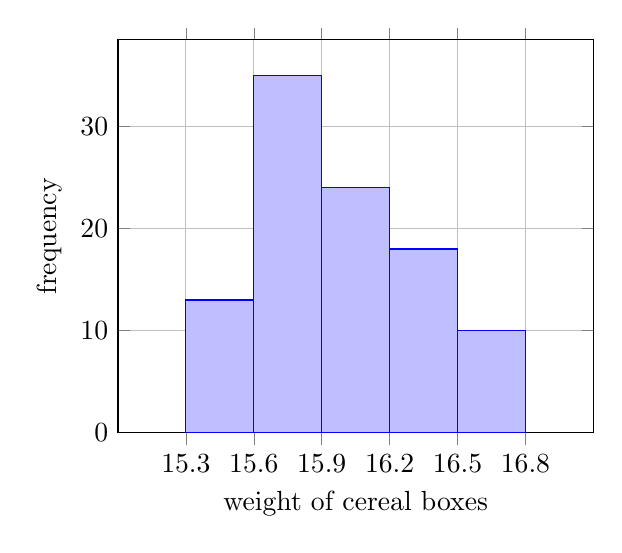
\begin{tikzpicture}[scale=1]
\begin{axis}[     
	ybar interval,
	x tick label as interval=false,    
	ymin=0,
	xmin=15,
	xmax=17.1,
	width=3in,
	%height=3in,
	grid=major,
	ylabel=frequency,
	xlabel=weight of cereal boxes
	] 
	\addplot [fill=blue!25,draw=blue] table [x=Lower, y=Count] { 
		Lower Upper Count 
		15.3 15.6 13
		15.6 15.9 35
		15.9 16.2 24
		16.2 16.5 18
		16.5 16.8 10
		16.8 17.1 0
	};
\end{axis}
\end{tikzpicture}
\par\end{centering}
\caption{\label{fig:Number-of-children}Weights of boxes of cereal.}
\end{figure}
\yspace\yspace
\end{enumerate}
\end{multicols}
\item Forty randomly selected families were surveyed to determine the number
of children in each family. The following results were found:

\hfill%
\begin{tabular}{cccccccc}
3.7  & 3.6 & 4.0 & 3.8 & 4.1 & 3.9 & 3.5 & 3.9\tabularnewline
3.6 & 4.0 & 3.6 & 3.7 & 3.9 & 3.3 & 3.6 & 4.0\tabularnewline
\end{tabular}\hfill\hspace{0cm}\begin{multicols}{2}
\begin{enumerate}
\item Find the mean.

\begin{enumerate}
\item []$\bar{x}=\frac{\sum x}{n}=\frac{60.2}{16}\approx3.7625$\vfill
\end{enumerate}
\item Find the median.

\begin{enumerate}
\item []$\frac{3.7+3.8}{2}=3.75$\vfill
\end{enumerate}
\item Find the standard deviation.

\begin{enumerate}
\item []$s=\sqrt{\frac{\sum(x-\bar{x})^{2}}{n-1}}\approx.2217$\vfill
\end{enumerate}
\item Construct a histogram using 5 subintervals, beginning at 3.2, and
ending at 4.2.\columnbreak
\item []\vspace{4cm}\begin{tikzpicture}[scale=.8]
\begin{axis}[     ybar,     ymin=0 ] 
\addplot +[hist={bins=5,data min=3.2,data max=4.2}] table [y index=0] {hist_data_cereal.csv}; 
\end{axis} 
\end{tikzpicture} 
\end{enumerate}
\end{multicols}\newpage
\item Tom and Jerry golfed five times during their vacation. Their scores
are given in the table below:

\hfill%
\begin{tabular}{cccccc}
\textbf{Tom}  & 103 & 99 & 107 & 93 & 92\tabularnewline
\textbf{Jerry} & 101 & 92 & 83 & 96 & 111\tabularnewline
\end{tabular}\hfill\hspace{0cm}
\begin{enumerate}[resume]
\item []Who is the more consistent golfer?

\begin{enumerate}[resume]
\item []Tom has a standard deviation of $s_{T}\approx6.4187$
\item []Jerry has a standard deviation of $s_{J}\approx10.4067$. So Tom
is more consistent since $6.41<10.40$.\vfill
\end{enumerate}
\end{enumerate}
\item A population is normally distributed with mean 78 and standard deviation
7.5.

\begin{enumerate}
\item Draw a sketch of the bell curve labeling the mean and the intervals
representing 1, 2, and 3 standard deviations of the mean.

\begin{enumerate}
\item []\normalcdf{78}{7.5}{55.5}{100.5}
\end{enumerate}
\item Find the percentage of data lies in each of the intervals.
\end{enumerate}
\end{enumerate}
\begin{multicols}{3}

\scalebox{0.9}{\normalcdf{78}{7.5}{70.5}{85.5}}

\scalebox{0.9}{\normalcdf{78}{7.5}{63}{93}}

\scalebox{0.9}{\normalcdf{78}{7.5}{55.5}{100.5}}

\end{multicols}\vfill
\begin{enumerate}[resume]
\item Find the following probabilities, 

\begin{enumerate}
\item $p(z<1.35)$\begin{multicols}{2}

\begin{enumerate}
\item []$p(z<1.35)\approx91.15\%$ \columnbreak
\item []\normalcdf{0}{1}{-4}{1.35}
\end{enumerate}
\end{multicols}\vfill
\item $p(0<z<2.02)$\begin{multicols}{2}

\begin{enumerate}
\item []$p(0<z<2.02)\approx47.83\%$ \columnbreak
\item []\normalcdf{0}{1}{0}{2.02}
\end{enumerate}
\end{multicols}\vfill
\item $p(-.09<z<1.06)$\begin{multicols}{2}

\begin{enumerate}
\item []$p(-.09<z<1.06)\approx39.13\%$ \columnbreak
\item []\normalcdf{0}{1}{-.09}{1.06}
\end{enumerate}
\end{multicols}\vfill
\item $p(-1.1<z<-.08)$\begin{multicols}{2}

\begin{enumerate}
\item []$p(-1.1<z<-.08)\approx33.25\%$ \columnbreak
\item []\normalcdf{0}{1}{-1.1}{-.08}
\end{enumerate}
\end{multicols}\vfill
\end{enumerate}
\item A population is normally distributed with a mean 78 and standard deviation
7.5. Find the following probabilities. 

\begin{enumerate}
\item $p(x<70)$\begin{multicols}{2}

\begin{enumerate}
\item []$z_{70}=\frac{70-78}{7.5}=-1.0\bar{6}\approx-1.07$
\item []$p(z<-1.07)\approx14.23\%$ \columnbreak
\item []\normalcdf{78}{7.5}{48}{70}
\end{enumerate}
\end{multicols}\vfill
\item $p(70<x<85)$\begin{multicols}{2}

\begin{enumerate}
\item []$z_{70}\approx-1.07$ and $z_{105}=\frac{85-78}{7.5}\approx.93$
\item []$p(-1.07<z<.93)$
\item []$=p(z<.93)-p(z<-1.07)\approx68.15\%$\columnbreak
\item []\normalcdf{78}{7.5}{70}{85}
\end{enumerate}
\end{multicols}\vfill
\item $p(80<x<95.5)$\begin{multicols}{2}

\begin{enumerate}
\item []$z_{80}=\frac{80-78}{7.5}\approx.27$ and $z_{95.5}=\frac{95.5-78}{7.5}\approx2.33$
\item []$p(.27<z<2.33)$
\item []$=p(z<2.33)-p(z<.27)\approx38.37\%$\columnbreak
\item []\normalcdf{78}{7.5}{80}{95.5}
\end{enumerate}
\end{multicols}\vfill
\item $p(95.5<x<108)$\begin{multicols}{2}

\begin{enumerate}
\item []$z_{95.5}\approx2.33$ and $z_{108}=\frac{108-78}{7.5}=4$
\item []$p(2.33<z<4)$
\item []$=p(z<4)-p(z<2.33)\approx0.99\%$\columnbreak
\item []\normalcdf{78}{7.5}{95.5}{108}
\end{enumerate}
\end{multicols}\vfill
\end{enumerate}
\item Find $c$ such that each of the following is true.

\begin{enumerate}
\item $p(z<c)=0.2776$\begin{multicols}{2}

\begin{enumerate}
\item []$\underset{\mbox{area}}{.2776}\rightarrow\underset{\mbox{z-score}}{-.59}$
\item []$c=-.59$\columnbreak
\item []\normalpdf{0}{1}{-4}{-.59}{-.59}
\end{enumerate}
\end{multicols}\vfill
\item $p(z>c)=.0351$$\leftarrow$area in right tail\begin{multicols}{2}

\begin{enumerate}
\item []Find \emph{z-}score for $1-.0351=.9649$
\item []$\underset{\mbox{area}}{.9649}\rightarrow\underset{\mbox{z-score}}{1.81}$
\item []$c=1.81$\columnbreak
\item []\normalpdf{0}{1}{1.81}{4}{1.81}
\end{enumerate}
\end{multicols}\vfill
\item $p(-c<z<c)=.733$\begin{multicols}{2}

\begin{enumerate}
\item []The area is split on either side of the mean,
\item []Area$=\frac{.733}{2}=.3665$
\item []$\underset{\mbox{area}}{.3665}\rightarrow\underset{\mbox{z-score}}{\pm1.11}$
(using Appendix F)
\item []$c=1.11$ \columnbreak
\item []\normalpdfB{0}{1}{-1.11}{1.11}
\end{enumerate}
\end{multicols}\vfill
\item Let $\mu=100$ and $\sigma=15$ find $c$ such that $p(x<c)=27.76\%$\begin{multicols}{2}

\begin{enumerate}
\item []$\underset{\mbox{area}}{.2776}\rightarrow\underset{\mbox{z-score}}{-.59}$
\item []$c=\sigma z+\mu\Rightarrow c=15(-.59)+100$
\item []$c=91.15$ \columnbreak
\item []\normalpdf{100}{15}{50}{91.15}{91.15}
\end{enumerate}
\end{multicols}\vfill
\end{enumerate}
\item The time it takes latex paint to dry is normally distributed with
$\mu=3.5$ hours and $\sigma=.75$ hours. Find the probability that
drying time will be as follows.

\begin{enumerate}
\item less than $2.25$ hours.\begin{multicols}{2}

\begin{enumerate}
\item []$z_{2.25}=\frac{2.25-3.5}{.75}=-1.6\bar{6}\approx-1.67$
\item []$p(x<2.25)=p(z<-1.67)=4.75\%$\columnbreak
\item []\normalcdf{3.5}{.75}{.5}{2.25}
\end{enumerate}
\end{multicols}\vfill
\end{enumerate}
\item The average score on the ACT is $18$ with a standard deviation of
$6$. If a college only wants to accept students with an ACT score
at least in the top 25\%. What is the minimum score they should accept?
What about the top 5\%?\begin{multicols}{2}

\begin{enumerate}
\item [\textbf{top 25\%:}]$\underset{\mbox{area}}{.75}\rightarrow\underset{\mbox{z-score}}{\approx.67}$
\item []$c=\sigma z+\mu\Rightarrow c=6(.68)+18$
\item []$c=22.08$ 
\item []\normalpdf{18}{6}{22.08}{42}{22.08}\columnbreak
\item [\textbf{top 5\%:}]$\underset{\mbox{area}}{.95}\rightarrow\underset{\mbox{z-score}}{\approx1.645}$
\item []$c=\sigma z+\mu\Rightarrow c=6(1.65)+18$
\item []$c=27.9$ 
\item []\normalpdf{18}{6}{27.9}{42}{27.9}\columnbreak
\end{enumerate}
\end{multicols}\vfill
\end{enumerate}

\end{document}
